\section{Results}

\subsection{Held-out test performance}
Table~\ref{tab:perf_gb_cnn} summarizes held-out test performance for the tuned Gradient Boosting (feature-based) classifier and the CNN1D (sequence-based) model. Precision/recall/F1 are reported for the chimeric class. The tuned Gradient Boosting model exhibits high precision (0.937) but lower recall (0.663), indicating a conservative decision strategy that reduced false positives at the expense of missed chimeric reads. In contrast, the CNN1D substantially increases recall (0.959) and overall discrimination (ROC--AUC 0.961), at the cost of reduced precision (0.872), resulting in more clean reads flagged as chimeric.

\begin{table}[htbp]
\centering
\caption{Held-out test performance of the tuned Gradient Boosting model and CNN1D. Precision/recall/F1 are reported for the chimeric (positive) class.}
\label{tab:perf_gb_cnn}
\begin{tabular}{|l|l|l|l|l|l|}
\hline
Model & Accuracy & Precision & Recall & F1 & ROC--AUC \\
\hline
Gradient Boosting (tuned) & 0.809 & 0.937 & 0.663 & 0.777 & 0.846 \\
CNN1D (final)             & 0.909 & 0.872 & 0.959 & 0.912 & 0.961 \\
\hline
\end{tabular}
\end{table}

\subsection{Error profiles}
The trade-off between the two models is visible in Fig.~\ref{fig:confmats}. Gradient Boosting produces relatively few false positives (179 clean reads predicted as chimeric) but many false negatives (1,348 chimeric reads predicted as clean). CNN1D reverses this pattern, with markedly fewer false negatives (165) but more false positives (561). These complementary error profiles motivate evaluating both models in terms of downstream assembly outcomes rather than classification metrics alone.

\begin{figure}[htbp]
  \centering
  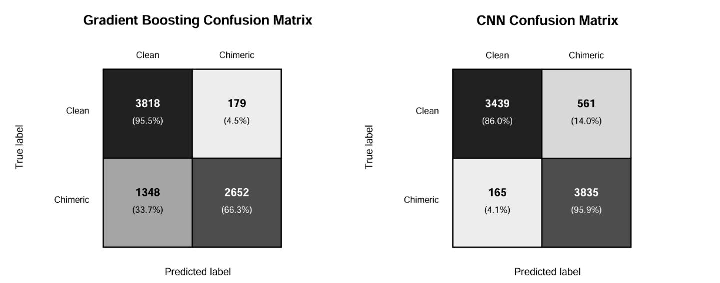
\includegraphics[width=0.85\textwidth]{../figures/confusion_matrices.pdf}
  \caption{Confusion matrices for the Gradient Boosting and CNN1D models on the held-out test.}
  \label{fig:confmats}
\end{figure}

\subsection{External Validation Under Varying Read Depths and Chimera Rates}
Table~\ref{tab:assembly_bandage} reports Bandage and SPAdes graph statistics for unfiltered and filtered assemblies across read depths and chimera rates. Filtering substantially reduces graph complexity under high chimera rates. At 20k reads and 50\% chimeras, the unfiltered assembly becomes extremely fragmented (966 nodes), whereas both GB and CNN1D restore near-contiguity (3 and 1 nodes, respectively). At 10k reads and 50\% chimeras, CNN1D collapses the graph to a single node, while GB reduces complexity to 2 nodes, consistent with CNN1D’s higher chimera recall and more aggressive removal of ambiguous read links. However, at low depth (3.2k), CNN1D occasionally increases fragmentation at higher chimera rates (15--50\%), suggesting that over-filtering can remove critical read support when coverage is marginal. Overall, GB provides a conservative approach for low-depth inputs, while CNN is most beneficial at moderate-to-high coverage and high chimeric rates. 

\begin{figure}[htbp]
  \centering
  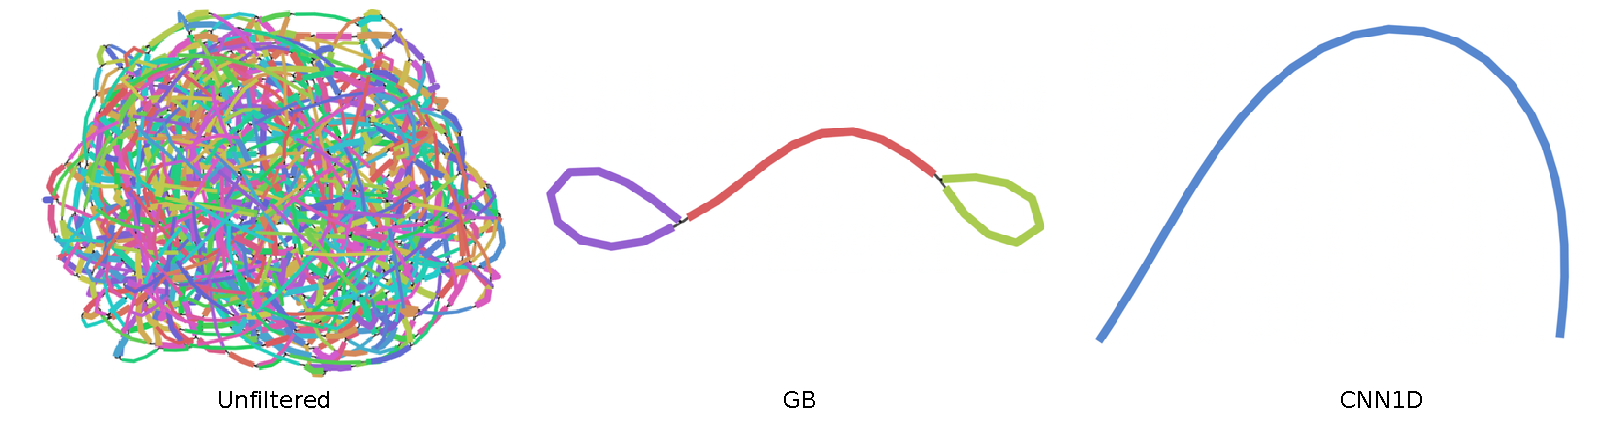
\includegraphics[width=0.95\textwidth]{figures/20k_50pct.pdf}
  \caption{Bandage assembly graphs for 20k reads with 50\% chimeras at a 50\% filtering threshold.}
  \label{fig:bandage_20k_50pct}
\end{figure}

\begin{figure}[htbp]
  \centering
  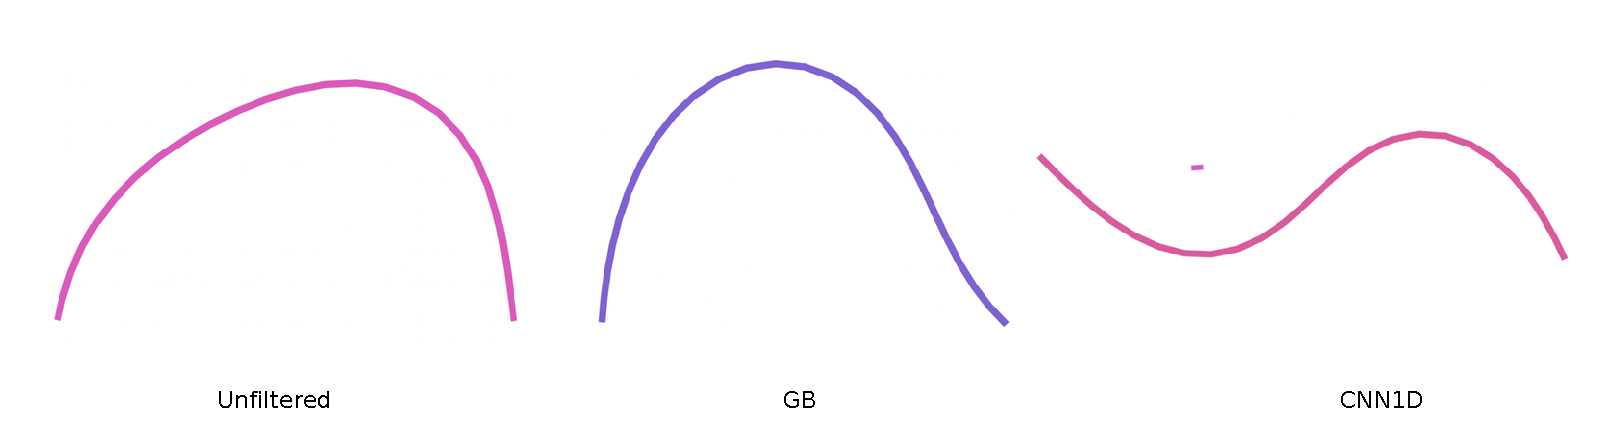
\includegraphics[width=0.95\textwidth]{figures/3200_50pct.pdf}
  \caption{Bandage assembly graphs for 3200 reads with 50\% chimeras at a 50\% filtering threshold.}
  \label{fig:bandage_3200_50pct}
\end{figure}


\begin{table}[t]
\centering
\caption{Assembly statistics for unfiltered and filtered reads across read depths and chimera rates. Nodes summarize graph complexity. Reads kept indicates the percentage of input reads retained after filtering. Max length is reported from SPAdes assemblies.}
\label{tab:assembly_bandage}
\scriptsize
\begin{tabular}{|l|l|l|l|l|l|}
\hline
Depth & Chimera\% & Condition & Nodes & Reads kept (\%) & Max length \\
\hline
\multirow{12}{*}{3.2k}
& 5  & Unfiltered & 2 & 100.000 & 16599 \\
& 5  & GB         & 1 & 97.406  & 16577 \\
& 5  & CNN        & 1 & 82.125  & 16575 \\
& 10 & Unfiltered & 1 & 100.000 & 16591 \\
& 10 & GB         & 1 & 95.219  & 16615 \\
& 10 & CNN        & 1 & 79.812  & 16590 \\
& 15 & Unfiltered & 1 & 100.000 & 16645 \\
& 15 & GB         & 1 & 93.375  & 16606 \\
& 15 & CNN        & 3 & 75.188  & 14925 \\
& 50 & Unfiltered & 1 & 100.000 & 16736 \\
& 50 & GB         & 1 & 77.875  & 16646 \\
& 50 & CNN        & 2 & 48.781  & 16247 \\
\hline
\multirow{12}{*}{10k}
& 5  & Unfiltered & 1 & 100.000 & 16615 \\
& 5  & GB         & 1 & 97.320  & 16615 \\
& 5  & CNN        & 1 & 83.090  & 16603 \\
& 10 & Unfiltered & 1 & 100.000 & 16704 \\
& 10 & GB         & 1 & 95.300  & 16614 \\
& 10 & CNN        & 1 & 78.470  & 16693 \\
& 15 & Unfiltered & 1 & 100.000 & 16735 \\
& 15 & GB         & 1 & 93.330  & 16642 \\
& 15 & CNN        & 1 & 75.950  & 16611 \\
& 50 & Unfiltered & 3 & 100.000 & 16715 \\
& 50 & GB         & 2 & 78.940  & 16787 \\
& 50 & CNN        & 2 & 49.470  & 16709 \\
\hline
\multirow{12}{*}{20k}
& 5  & Unfiltered & 1   & 100.000 & 16669 \\
& 5  & GB         & 2   & 97.490  & 16619 \\
& 5  & CNN        & 1   & 82.575  & 16669 \\
& 10 & Unfiltered & 3   & 100.000 & 16799 \\
& 10 & GB         & 1   & 95.135  & 16616 \\
& 10 & CNN        & 1   & 78.935  & 16616 \\
& 15 & Unfiltered & 3   & 100.000 & 16747 \\
& 15 & GB         & 1   & 93.345  & 16891 \\
& 15 & CNN        & 1   & 75.220  & 16646 \\
& 50 & Unfiltered & 966 & 100.000 & 407 \\
& 50 & GB         & 3   & 78.485  & 16799 \\
& 50 & CNN        & 1   & 49.890  & 16745 \\
\hline
\end{tabular}
\end{table}

\FloatBarrier